\section{Solución propuesta}
\label{sec:solucion_propuesta}

\subsection{Características de la solución}
\label{subsec:caracteristicas-solucion}
La solución consiste en incorporar un módulo en NEURONE \parencite{gonzalez2017neurone} que clasifique y prediga de forma continua el desempeño de búsqueda de los estudiantes de enseñanza básica en un curso de alfabetización informacional, específicamente en el tema de investigaciones en línea\footnote{\traduccionlibre} (\ingles{online inquiry}). 

Los datos son recopilados y almacenados por NEURONE, estos datos provienen de registros del proceso de búsqueda de información en línea en un sistema cerrado, los cuales son: historial de navegación, consultas realizadas, movimientos del \ingles{mouse}, escritura por teclado, número de \ingles{clicks} y tiempos de permanencia en páginas \ingles{web}. Además, se conoce con anticipación los documentos y párrafos ideales a seleccionar por parte de los estudiantes.

El módulo propuesto hará uso de Apache Spark\footnote{https://spark.apache.org/}, el cual es un \ingles{framework} de código abierto para el procesamiento de datos masivos, el cual incluye librerías de minería de datos y aprendizaje de máquina. Este módulo se conectará con el sistema NEURONE, funcionando como una extensión del mismo, consultando su base de datos, alimentando y perfeccionando el modelo. 

El ciclo de construcción, evaluación y optimización del modelo se ilustra en la Figura \ref{fig:ml-pipeline}, donde a través de los datos históricos obtenidos de NEURONE construye el modelo, lo evalúa y lo optimiza en un proceso continuo, entregando como resultado la clasificación del desempeño de búsqueda y prediciendo de forma continua a partir del comportamiento actual de búsqueda de información del estudiante.

%Fuente: https://tex.stackexchange.com/questions/4338/correctly-scaling-a-tikzpicture
\begin{figure}[H]
	\centering
	%FIX: dont compile
	%\scalebox{0.8}{%\centering\makebox[\textwidth]{
\begin{tikzpicture}[node distance=3cm, auto]

    % Place nodes
    \node[label={Estudiante},charlie,monitor,minimum size=1.3cm] (estudiante);
    \node[block, right of=estudiante] (data-ingestion) {Entrada de datos};
    \node[block, right of=data-ingestion] (data-clean) {Transformación de datos};
    \node[block, right of=data-clean] (model-training) {Entrenamiento del modelo};
    \node[block, right of=model-training] (model-testing) {Evaluación del modelo};
    \node[block, right of=model-testing] (prediction) {Predicción};

\draw[line] (estudiante) -- (data-ingestion)
            (data-ingestion) -- (data-clean)
            (data-clean) -- (model-training)
            (model-training) -- (model-testing)
            (model-testing) -- (prediction);

\path[line,dashed] 
   (model-testing.south) -- +(0,-.35) -| (model-training.south)
   (prediction.south) -- +(0,-.60) -| (data-ingestion.south);

\coordinate[below=11mm of data-ingestion] (bottom brace);

\draw [my brace]
      (data-ingestion.south|-bottom brace) -- (model-training.south west|-bottom brace) 
      node[bottom label] {
        %Obtención de datos de NEURONE
        \begin{itemize}
        \item Spark
        \end{itemize}
      };

\draw [my brace]
      (model-training.south|-bottom brace) -- (prediction.south west|-bottom brace) 
      node[bottom label] {
        %Environmental \& Human factors
        \begin{itemize}
        \item Spark ML
        \end{itemize}
      };


\end{tikzpicture}
%}
	%\resizebox{1.0\textwidth}{!}{%\centering\makebox[\textwidth]{
\begin{tikzpicture}[node distance=3cm, auto]

    % Place nodes
    \node[label={Estudiante},charlie,monitor,minimum size=1.3cm] (estudiante);
    \node[block, right of=estudiante] (data-ingestion) {Entrada de datos};
    \node[block, right of=data-ingestion] (data-clean) {Transformación de datos};
    \node[block, right of=data-clean] (model-training) {Entrenamiento del modelo};
    \node[block, right of=model-training] (model-testing) {Evaluación del modelo};
    \node[block, right of=model-testing] (prediction) {Predicción};

\draw[line] (estudiante) -- (data-ingestion)
            (data-ingestion) -- (data-clean)
            (data-clean) -- (model-training)
            (model-training) -- (model-testing)
            (model-testing) -- (prediction);

\path[line,dashed] 
   (model-testing.south) -- +(0,-.35) -| (model-training.south)
   (prediction.south) -- +(0,-.60) -| (data-ingestion.south);

\coordinate[below=11mm of data-ingestion] (bottom brace);

\draw [my brace]
      (data-ingestion.south|-bottom brace) -- (model-training.south west|-bottom brace) 
      node[bottom label] {
        %Obtención de datos de NEURONE
        \begin{itemize}
        \item Spark
        \end{itemize}
      };

\draw [my brace]
      (model-training.south|-bottom brace) -- (prediction.south west|-bottom brace) 
      node[bottom label] {
        %Environmental \& Human factors
        \begin{itemize}
        \item Spark ML
        \end{itemize}
      };


\end{tikzpicture}
%}}
	%Este funciona
	%%\centering\makebox[\textwidth]{
\begin{tikzpicture}[node distance=3cm, auto]

    % Place nodes
    \node[label={Estudiante},charlie,monitor,minimum size=1.3cm] (estudiante);
    \node[block, right of=estudiante] (data-ingestion) {Entrada de datos};
    \node[block, right of=data-ingestion] (data-clean) {Transformación de datos};
    \node[block, right of=data-clean] (model-training) {Entrenamiento del modelo};
    \node[block, right of=model-training] (model-testing) {Evaluación del modelo};
    \node[block, right of=model-testing] (prediction) {Predicción};

\draw[line] (estudiante) -- (data-ingestion)
            (data-ingestion) -- (data-clean)
            (data-clean) -- (model-training)
            (model-training) -- (model-testing)
            (model-testing) -- (prediction);

\path[line,dashed] 
   (model-testing.south) -- +(0,-.35) -| (model-training.south)
   (prediction.south) -- +(0,-.60) -| (data-ingestion.south);

\coordinate[below=11mm of data-ingestion] (bottom brace);

\draw [my brace]
      (data-ingestion.south|-bottom brace) -- (model-training.south west|-bottom brace) 
      node[bottom label] {
        %Obtención de datos de NEURONE
        \begin{itemize}
        \item Spark
        \end{itemize}
      };

\draw [my brace]
      (model-training.south|-bottom brace) -- (prediction.south west|-bottom brace) 
      node[bottom label] {
        %Environmental \& Human factors
        \begin{itemize}
        \item Spark ML
        \end{itemize}
      };


\end{tikzpicture}
%}
	%\input{03_GraphicFiles/p06.pdf}
	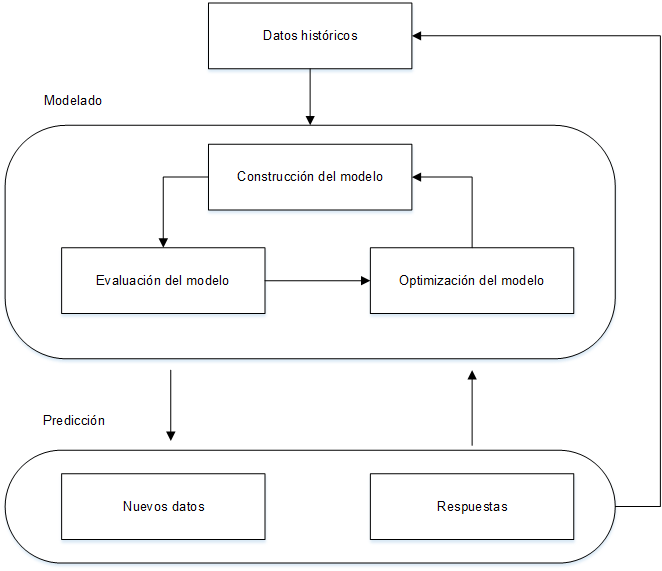
\includegraphics[width=0.7\textwidth]{03_GraphicFiles/p06.png}
	\captionsource{Ciclo de construcción y perfecionamiento del modelo}{\fuentePropia}
	\label{fig:ml-pipeline}
\end{figure}


\subsection{Propósito de la solución}
\label{subsec:proposito-solucion}
El propósito de la solución consiste en proveer evaluaciones de desempeño de búsqueda oportunas que permitan a los docentes aplicar acciones correctivas durante el proceso de formación y desarrollo de competencias informacionales en cursos de alfabetización informacional.

Con el módulo propuesto en este trabajo, el docente obtiene una estimación temprana del desempeño del estudiante en el proceso de búsqueda de información, de tal forma que él pueda guiar al estudiante en el proceso. Tal como ilustra la Figura \ref{fig:docente_estudiante}, el estudiante interactúa con el sistema educacional, en este caso NEURONE y la plataforma propuesta a través de técnicas de minería de datos informa al docente de los patrones y predicciones del desempeño de búsqueda del estudiante con el objetivo de ayudar en la toma de decisiones al docente correspondiente para diseñar y planificar de mejor forma la entrega de contenidos hacia el estudiante.

\begin{figure}[H]
	\centering
	%\begin{tikzpicture}[node distance=3.5cm]

%\matrix(m)[matrix of nodes,row sep=3em,column sep=4em,minimum width=2em]{
%	\node[label={Docente}, businessman, minimum size=1.5cm](docente); & \node[label={Estudiante}, charlie, mirrored, monitor,minimum size=1.5cm](estudiante);\\
%};


\node[label={Estudiante},charlie,monitor,minimum size=1.5cm](estudiante);
%motor de busqueda
\node(db)[cylinder, 
        shape border rotate=90, 
        draw,
        minimum height=1.5cm,
        minimum width=2cm,
        shape aspect=.25,
        right=of estudiante] {Motor de búsqueda};

\node[label={Docente},businessman,monitor,mirrored,minimum size=1.5cm,right=of db](docente);


% Draw edges
\draw[arrow] (estudiante) -- (db);
%\draw[arrow] (db) -- (estudiante);
\draw[arrow] (db) -- (docente);

%\draw[->] (B.west) +(0,-1em) coordinate (b1) -- (A.east |- b1);
%\draw[->] (db.west) +(0,-1em) coordinate (b1) -- (A.east |- b1);

\end{tikzpicture}
	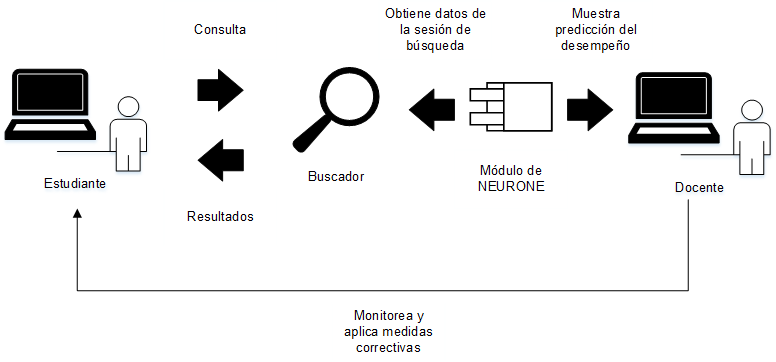
\includegraphics[width=0.9\textwidth]{03_GraphicFiles/monitor.png}
	%\input{03_GraphicFiles/p07.pdf}
	\captionsource{Proceso de búsqueda de información de un estudiante}{\fuentePropia}
	\label{fig:docente_estudiante}
\end{figure}
